\documentclass[letterpaper,12pt]{report}
\usepackage[utf8]{inputenc}
\usepackage{amsmath}
\usepackage[x11names]{xcolor}
\usepackage{pgfplots}
\usepackage{bm}

\usetikzlibrary{arrows.meta, angles, quotes}
\pgfplotsset{
  compat = newest,
  my_style/.style={
    clip=false,
    axis lines=middle,
    axis equal,
    axis line style={Latex-Latex},
    xmin=-1,
    xmax=1.5,
    ymin=-1,
    ymax=1.5,
    xlabel={$x$},
    ylabel={$y$},
    xtick distance=1,
    ytick distance=1,
    line width=1pt,
  },
}

% MACROS %
\newcommand{\uvec}[1]{\boldsymbol{\hat{\textbf{#1}}}}

\begin{document}

To illustrate that $T$ is linear, let's show that it respects addition and scalar multiplication i.e. for two vectors $\vec{v}$ and $\vec{w}$ and a scalar $k$, the following holds true:
\begin{align*}
  T(\vec{v} + \vec{w}) &= T(\vec{v}) + T(\vec{w}) \\
  T(k\vec{v}) &= kT(\vec{v})
\end{align*}

First, show addition. Let $\vec{v} = \uvec{\i}$ and $\vec{w} = \uvec{\j}$. \\
% \begin{align*}
%   \vec{v} + \vec{w} = \uvec{\i} + \uvec{\j}
%   = \begin{bmatrix}
%     1 \\ 0
%   \end{bmatrix} + \begin{bmatrix}
%     0 \\ 1
%   \end{bmatrix}
%   = \begin{bmatrix}
%     1 \\ 1
%   \end{bmatrix}
% \end{align*} \\
\begin{tikzpicture}
  \begin{axis}[my_style]
    \addplot[Latex-Latex, black, domain=-0.75:1.5]{1/3 * x} node[right,pos=1] {$L$};

    \addplot[-Latex, DodgerBlue2] coordinates {
      (0, 0)
      (1, 0)
    } node[above,pos=1] {$\uvec{\i}$};
    \addplot[-Latex, PaleVioletRed3] coordinates {
      (0, 0)
      (0, 1)
    } node[right,pos=1] {$\uvec{\j}$};
    \addplot[-Latex, SeaGreen3] coordinates {
      (0, 0)
      (1, 1)
    } node[right,pos=1] {$\uvec{\i} + \uvec{\j}$};

    % Nodes to calculate the angle
    \path
      (3, 0)node(A){}
      (0, 0)node(B){}
      (3, 1)node(C){};
  \end{axis}

  \pic[draw, -, angle radius=10mm, angle eccentricity=1.2, "$\theta$", font=\tiny] {angle = A--B--C};
\end{tikzpicture}
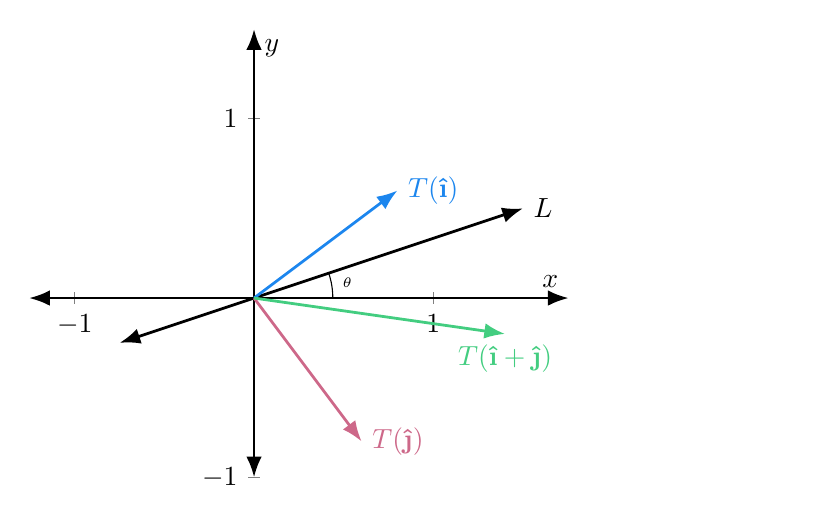
\begin{tikzpicture}
  \begin{axis}[my_style]
    \addplot[Latex-Latex, black, domain=-0.75:1.5]{1/3 * x} node[right,pos=1] {$L$};

    % theta = arccos(3/sqrt(10)) ≈ 0.32175 radians
    % | 0.8  0.6 |
    % | 0.6 -0.8 |
    \addplot[-Latex, DodgerBlue2] coordinates {
      (0, 0)
      (0.8, 0.6)
    } node[right,pos=1] {$T(\uvec{\i})$};
    \addplot[-Latex, PaleVioletRed3] coordinates {
      (0, 0)
      (0.6, -0.8)
    } node[right,pos=1] {$T(\uvec{\j})$};
    \addplot[-Latex, SeaGreen3] coordinates {
      (0, 0)
      (0.8+0.6, 0.6-0.8)
    } node[below,pos=1] {$T(\uvec{\i} + \uvec{\j})$};

    % Nodes to calculate the angle
    \path
      (3, 0)node(A){}
      (0, 0)node(B){}
      (3, 1)node(C){};
  \end{axis}

  \pic[draw, -, angle radius=10mm, angle eccentricity=1.2, "$\theta$", font=\tiny] {angle = A--B--C};
\end{tikzpicture} \\
To plot the vector sum $T(\uvec{\i}) + T(\uvec{\j})$, place the vectors head to tail and then draw a vector from the free tail to the free head. \\
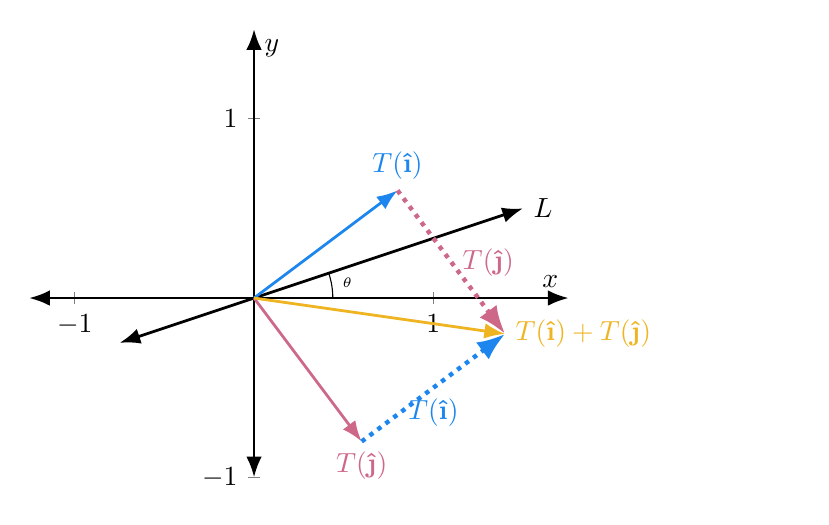
\begin{tikzpicture}
  \begin{axis}[my_style]
    \addplot[Latex-Latex, black, domain=-0.75:1.5]{1/3 * x} node[right,pos=1] {$L$};

    \addplot[-Latex, DodgerBlue2] coordinates {
      (0, 0)
      (0.8, 0.6)
    } node[above,pos=1] {$T(\uvec{\i})$};
    \addplot[-Latex, PaleVioletRed3] coordinates {
      (0, 0)
      (0.6, -0.8)
    } node[below,pos=1] {$T(\uvec{\j})$};

    \addplot[-Latex, DodgerBlue2, ultra thick, dotted] coordinates {
      (0.6, -0.8)
      (0.8+0.6, 0.6-0.8)
    } node[below, midway] {$T(\uvec{\i})$};
    \addplot[-Latex, PaleVioletRed3, ultra thick, dotted] coordinates {
      (0.8, 0.6)
      (0.8+0.6, 0.6-0.8)
    } node[right, midway] {$T(\uvec{\j})$};

    \addplot[-Latex, Goldenrod2] coordinates {
      (0, 0)
      (0.8+0.6, 0.6-0.8)
    } node[right,pos=1] {$T(\uvec{\i}) + T(\uvec{\j})$};

    % Nodes to calculate the angle
    \path
      (3, 0)node(A){}
      (0, 0)node(B){}
      (3, 1)node(C){};
  \end{axis}

  \pic[draw, -, angle radius=10mm, angle eccentricity=1.2, "$\theta$", font=\tiny] {angle = A--B--C};
\end{tikzpicture} \\
Compare the plots and observe that $T(\uvec{\i} + \uvec{\j}) = T(\uvec{\i}) + T(\uvec{\j})$. Thus, $T$ respects addition.

\newpage
Next show scalar multiplication. Let $k = 2$. \\
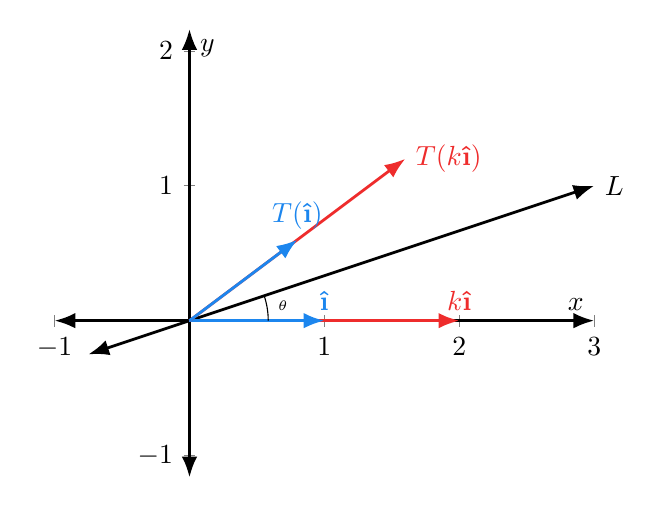
\begin{tikzpicture}
  \begin{axis}[
    my_style,
    xmin=-1,
    xmax=3,
    ymin=-1,
    ymax=2,
  ]
    \addplot[Latex-Latex, black, domain=-0.75:3]{1/3 * x} node[right,pos=1] {$L$};

    \addplot[-Latex, Firebrick2] coordinates {
      (0, 0)
      (2, 0)
    } node[above,pos=1] {$k\uvec{\i}$};
    \addplot[-Latex, DodgerBlue2] coordinates {
      (0, 0)
      (1, 0)
    } node[above,pos=1] {$\uvec{\i}$};

    % theta = arccos(3/sqrt(10)) ≈ 0.32175 radians
    % | 0.8  0.6 |
    % | 0.6 -0.8 |
      \addplot[-Latex, Firebrick2] coordinates {
      (0, 0)
      (1.6, 1.2)
    } node[right,pos=1] {$T(k\uvec{\i})$};
    \addplot[-Latex, DodgerBlue2] coordinates {
      (0, 0)
      (0.8, 0.6)
    } node[above,pos=1] {$T(\uvec{\i})$};

    % Nodes to calculate the angle
    \path
      (3, 0)node(A){}
      (0, 0)node(B){}
      (3, 1)node(C){};
  \end{axis}

  \pic[draw, -, angle radius=10mm, angle eccentricity=1.2, "$\theta$", font=\tiny] {angle = A--B--C};
\end{tikzpicture} \\
Let's simply multiply $T(\uvec{\i})$ by $k$ and plot that: \\
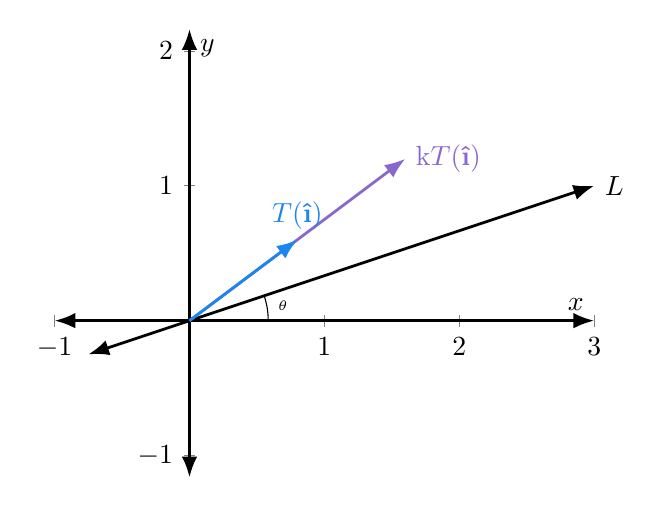
\begin{tikzpicture}
  \begin{axis}[
    my_style,
    xmin=-1,
    xmax=3,
    ymin=-1,
    ymax=2,
  ]
    \addplot[Latex-Latex, black, domain=-0.75:3]{1/3 * x} node[right,pos=1] {$L$};

    % theta = arccos(3/sqrt(10)) ≈ 0.32175 radians
    % | 0.8  0.6 |
    % | 0.6 -0.8 |
    \addplot[-Latex, MediumPurple3] coordinates {
      (0, 0)
      (1.6, 1.2)
    } node[right,pos=1] {k$T(\uvec{\i})$};
    \addplot[-Latex, DodgerBlue2] coordinates {
      (0, 0)
      (0.8, 0.6)
    } node[above,pos=1] {$T(\uvec{\i})$};

    % Nodes to calculate the angle
    \path
      (3, 0)node(A){}
      (0, 0)node(B){}
      (3, 1)node(C){};
  \end{axis}

  \pic[draw, -, angle radius=10mm, angle eccentricity=1.2, "$\theta$", font=\tiny] {angle = A--B--C};
\end{tikzpicture} \\
Compare the plots and observe that $T(k\uvec{\i}) = kT(\uvec{\i})$. Thus, $T$ respects scalar multiplication.

\newpage
The matrix $T$ in terms of $\theta$ is
\begin{align*}
  T_{\theta}(\vec{x}) =
  \begin{bmatrix}
    \cos{2\theta} & \sin{2\theta} \\
    \sin{2\theta} & -\cos{2\theta}
  \end{bmatrix}
\end{align*}
It can be found by observing the results of applying the transformation to $\uvec{\i}$ and $\uvec{\j}$:
\begin{align*}
  T(\uvec{\i}) &= \begin{bmatrix}
    \cos{2\theta} \\ \sin{2\theta}
  \end{bmatrix} \\
  T(\uvec{\j}) &= \begin{bmatrix}
    \sin{2\theta} \\ -\cos{2\theta}
  \end{bmatrix}
\end{align*}
% \begin{tikzpicture}
%   \begin{axis}[my_style]
%     \addplot[Latex-Latex, black, domain=-0.75:1.5]{1/3 * x} node[right,pos=1] {$L$};

%     \addplot[-Latex, DodgerBlue2] coordinates {
%       (0, 0)
%       (1, 0)
%     } node[above,pos=1] {$\uvec{\i}$};
%     \addplot[-Latex, PaleVioletRed3] coordinates {
%       (0, 0)
%       (0, 1)
%     } node[right,pos=1] {$\uvec{\j}$};

%     % theta = arccos(3/sqrt(10)) ≈ 0.32175 radians
%     % | 0.8  0.6 |
%     % | 0.6 -0.8 |
%     \addplot[-Latex, DodgerBlue2] coordinates {
%       (0, 0)
%       (0.8, 0.6)
%     } node[above,pos=1] {$T(\uvec{\i})$};
%     \addplot[-Latex, PaleVioletRed3] coordinates {
%       (0, 0)
%       (0.6, -0.8)
%     } node[right,pos=1] {$T(\uvec{\j})$};

%     % Nodes to calculate the angle
%     \path
%       (3, 0)node(A){}
%       (0, 0)node(B){}
%       (3, 1)node(C){};

%     % 2theta
%     \path
%       (0.8, 0)node(D){}
%       (0.8, 0.6)node(E){};
%   \end{axis}

%   \pic[draw, -, angle radius=10mm, angle eccentricity=1.2, "$\theta$", font=\tiny] {angle = A--B--C};
%   \pic[draw, DodgerBlue2, -, angle radius=15mm, angle eccentricity=1.2, "$2\theta$", font=\tiny, pic text options={shift={(-2pt,7pt)}}] {angle = D--B--E};
% \end{tikzpicture} \\
Setting those results as columns of a $2 \times 2$ matrix would give a matrix that produces those results:
\begin{align*}
  \begin{bmatrix}
    \cos{2\theta} & \sin{2\theta} \\
    \sin{2\theta} & -\cos{2\theta}
  \end{bmatrix}
  \begin{bmatrix}
    1 \\ 0
  \end{bmatrix} &=
  \begin{bmatrix}
    \cos{2\theta} \\ \sin{2\theta}
  \end{bmatrix} \\
  \begin{bmatrix}
    \cos{2\theta} & \sin{2\theta} \\
    \sin{2\theta} & -\cos{2\theta}
  \end{bmatrix}
  \begin{bmatrix}
    0 \\ 1
  \end{bmatrix} &=
  \begin{bmatrix}
    \sin{2\theta} \\ -\cos{2\theta}
  \end{bmatrix}
\end{align*}
\end{document}
